% Canonical, editable manuscript. All prose, equations, and tables are in this file.
% Build: latexmk -pdf -interaction=nonstopmode -halt-on-error main.tex
% Development study; original held-out restoration goals remain untested.
\documentclass[runningheads,orivec]{llncs}
\usepackage[T1]{fontenc}
\usepackage[utf8]{inputenc}
\usepackage{newtxtext}
\usepackage[varvw]{newtxmath}
\usepackage{graphicx}
\usepackage{booktabs}
\usepackage{float}
\usepackage{microtype}
\usepackage[hidelinks]{hyperref}
\hypersetup{pdfauthor={Alexander V. Mantzaris and James H. Korris},pdftitle={Checking Sound and Action: Generative AI for Underwater Acoustic Analysis},pdfsubject={Development study of acoustic correction and GPU agent comparisons}}

\begin{document}
\raggedbottom
\title{Checking Sound and Action: Generative AI for Underwater Acoustic Analysis}
\titlerunning{Checking Sound and Action in Underwater Acoustics}
\author{Alexander V. Mantzaris\inst{1} \and James H. Korris\inst{2}}
\authorrunning{A. V. Mantzaris and J. H. Korris}
\institute{Dr. Yvette Kanouff School of Data,\\
Mathematical, and Statistical Sciences\\
UCF, 4000 University Blvd, Orlando, FL 32816, USA\\
\email{alexander.mantzaris@ucf.edu}
\and
Creative Technologies Inc.\\
\email{james.korris@cretecinc.com}}
\maketitle


\begin{abstract}
Reliable underwater acoustic assistance requires numerical stability, acoustic fidelity, and verified execution of analysis actions. We present a reproducible evaluation protocol that separates these requirements across two tasks, waveform repair and tool-using assistance. A matched change to established velocity prediction removes severe diffusion instability and reduces combined reconstruction error by about 25\% on 64 reserved development cases, although a learned baseline remains better. On 32 agent tasks, reasoning yields 25 correct cue labels versus 16 for direct action selection, yet completes four tasks versus ten. A configuration gate eliminates six infeasible applied changes on sixteen new recordings, while completion rises only from two to three. Additional thinking improves setting correctness. Workflow comparisons and completion gains remain statistically inconclusive. The contribution combines preservation of recorded evidence, controlled interventions, and replayable execution records to identify which failures each remedy resolves and which persist. This supports decisions about model improvement, selective release, and configuration checks. Results concern development recordings. Vessel identification and physical control remain untested.
\keywords{Generative AI \and Passive acoustics \and Audio inpainting \and Reasoning agents \and Operator decision support}
\end{abstract}

\section{Evaluating sound and action}

An operator examining a low tone interrupted by missing audio must distinguish recorded evidence from a generated fill and a recommended setting from an executed action. Vessel recordings contain low-frequency and broadband structure \cite{veirs}, so plausible sound or correct cue labels alone cannot establish useful repair or completed analysis.

\textbf{Evaluation protocol.} We separate numerical stability, acoustic fidelity, and verified execution. Each task preserves recorded evidence, measures failures against explicit references or rules, and tests a targeted intervention under matched conditions. Component improvements are then checked against required outcomes. Repair and agent tasks are evaluated independently. Agents receive recorded context only, without an integrated repair-to-agent experiment.

\textbf{Contributions.} Controlled repair experiments distinguish numerical failure from remaining acoustic error and assess release feasibility. A comparison of four neural workflows separates cue labels, applied settings, and verified completion. Frozen inputs, prompts, tool returns, and scoring code support replay of all 208 scored agent episodes.

\begin{figure}[!ht]
\centering
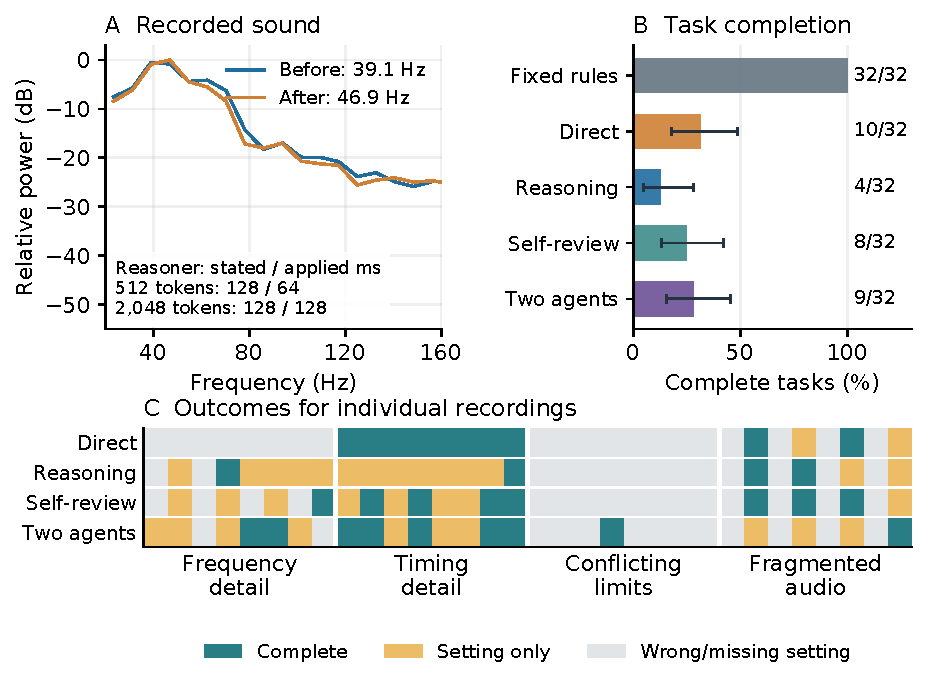
\includegraphics[width=\linewidth]{gpu_agent_comparison.pdf}
\caption{Recorded sound and executed decisions. (A) Before/after spectra at 128 ms, excluding gap frames. The callout compares stated/applied windows. (B) Complete tasks with 95\% Wilson intervals for neural workflows. (C) Individual recordings, with orange indicating correct settings but incomplete tasks. Two agents means planner--reviewer.}
\label{fig:configuration}
\end{figure}

In Fig.~\ref{fig:configuration}, the reasoner recommends 128 ms but applies 64 ms. Additional thinking corrects this case. The paired completion gain remains inconclusive.

\section{Related work and recordings}

Prior work generates and repairs general audio \cite{diffwave,csdi,moliner,simdps} and underwater spectrograms \cite{tembo}, estimates uncertainty \cite{cohen}, and calibrates risk \cite{ltt}. We use established velocity prediction \cite{salimans} to test how correcting numerical instability changes acoustic reconstruction and release feasibility.

Tool-based reasoning \cite{react}, self-review \cite{reflexion}, and multi-agent conversations \cite{autogen} are established. Li et al.\ \cite{signals_evidence} connect acoustic representations to a language model for detection reports. Our bounded tool task checks reported choices against measurements, applied settings, and verification under controlled interventions.

UniqueShip v1 \cite{uniqueship} contains 43,208 mono recordings, twelve classes, and 60.008 hours at an audited 32 kHz. Related recordings stay in one partition. Table~\ref{tab:1} separates generator training (G), quality-checker training (D), development (V), calibration (C), and final testing. Actual C/test outcomes remain unopened.

\begin{table}[htbp]
\caption{Audited source partitions. Counts describe available data, not evaluated outcomes.}
\label{tab:1}
\centering\small
\begin{tabular*}{\linewidth}{@{\extracolsep{\fill}}lrrr@{}}
\toprule

\textbf{Partition} & \textbf{Sources} & \textbf{Groups} & \textbf{Pilot use} \\

\midrule

G & 26,321 & 2,996 & 1,440 sources \\

D & 3,962 & 467 & 200 groups \\

V & 4,445 & 400 & 200 groups \\

C & 4,003 & 547 & Unopened \\

Test & 4,477 & 610 & Unopened \\

\bottomrule
\end{tabular*}
\end{table}

Background groups use hydrophone/date, pooling unknown devices by date. No duplicate files or cross-partition groups are found. However, 1,332/1,522 dates span partitions, leaving environmental independence unproven. Excerpts are 4.096 s at 8 kHz, with gaps erased after resampling. Twelve shorter clips are excluded.

\section{Repair the gap, preserve the evidence}

The repair pipeline compares four diffusion proposals with a deterministic learned baseline B. An observation-only quality predictor selects a proposal. A calibrated release rule accepts it or retains B as output P. All filled samples remain marked as estimates, including baseline fills.

\textbf{Preserve recorded evidence.} Let $m=1$ on recorded samples and $m=0$ in gaps, with $y=m\odot x$ the available audio. Every generation step restores recorded samples through the projection
\begin{equation}
\Pi_y(z)=m\odot y+(1-m)\odot z.\label{eq:projection}
\end{equation}
Mean and root-mean-square scaling use recorded samples only, with a training-fixed floor. Inverse scaling preserves those samples exactly for later inspection.

Gaps last 50/100/250/500 ms, with at least 0.75 s context per side. Two nearby recorded segments are hidden as self-supervised probes, withholding their answers from each repair. Four proposals and two probe repairs at 32 DDIM steps \cite{ddim} require 192 model evaluations. Hidden gap references and vessel annotations never enter generation.

A predictor fitted on 200 D groups ranks proposals using agreement, baseline differences, boundaries, and probe errors. Duration and dispersion gate controls retain the full selector.

\textbf{Measure the missing part.} We combine normalized waveform error (NMSE) with frequency-pattern error (spectral convergence, SC):
\begin{equation}
Q=\tfrac12\min\!\left(\frac{\mathrm{NMSE}_{\mathrm{gap}}}{4},1\right)+\tfrac12\min\!\left(\frac{\mathrm{SC}_{\mathrm{gap}}}{2},1\right).\label{eq:quality}
\end{equation}
Lower Q is better. NMSE measures waveform error relative to true gap energy. SC compares frequency magnitudes at three scales. A proposal is worse if Q exceeds B's by over 0.02. These scores assess repair quality without establishing identification confidence.

The release rule seeks at most 10\% worse fills using confidence bounds \cite{ltt}, assuming independent groups and matching distributions. Zero acceptances disable release without certifying quality.

\textbf{Implementation.} A 2.72-million-parameter DiffWave adaptation uses a 1,000-step cosine schedule \cite{nichol}, seed 17, batch 16, and 5,000 updates on 1,440 G sources. The same-backbone baseline trains for 2,500 updates with waveform and spectral losses. Both use an RTX 4090, with configurations preserved.

\section{Testing whether candidate quality supports release}

Starting at the final noise step produces enormous errors on four G recordings. Before development evaluation, an amendment starts at step 934, the last with at least 1\% signal power, and limits generated amplitudes. This approximate Gaussian initialization \cite{lin} defines the original amended sampler.

V assigns 64 groups each to tuning, practice calibration, and reserved evaluation, leaving eight unused. The first 32 tuning groups also monitor training. Even retrospective best-of-four selection improves on B by 0.02 in only 5/64 tuning groups (7.8\%). This misses the predeclared 20\% feasibility threshold. Doubling generation steps leaves the count unchanged, so the original main study stops.

\begin{table}[htbp]
\caption{Repair on 64 reserved development groups. Lower error is better. AI use gives diffusion coverage. Worse means Q exceeds B's by over 0.02. Calls lists diffusion evaluations (one baseline pass for B). Velocity rows are ungated (Sect.~\ref{sec:correction}).}
\label{tab:2}
\centering\small
\begin{tabular*}{\linewidth}{@{\extracolsep{\fill}}lrrrrr@{}}
\toprule

\textbf{Output} & \textbf{Error Q} & \textbf{NMSE} & \textbf{AI use} & \textbf{Worse} & \textbf{Calls} \\

\midrule

Zero fill & 0.375 & 1.000 & 0.00 & --- & 0 \\

Linear interpolation & 0.314 & 1.021 & 0.00 & --- & 0 \\

Baseline fill B & 0.239 & 0.713 & 0.00 & --- & 0 \\

One AI proposal (C1) & 0.412 & 2.274 & 1.00 & 0.891 & 32 \\

Central of four (C2) & 0.404 & 1.949 & 1.00 & 0.891 & 128 \\

Always use selected AI (C3) & 0.349 & 1.460 & 1.00 & 0.812 & 192 \\

Checked output P & 0.239 & 0.713 & 0.00 & 0.000 & 192 \\

\midrule

Velocity: old sampler & 0.318 & 1.313 & 1.00 & 0.781 & 32 \\

Velocity: one draw & 0.308 & 1.251 & 1.00 & 0.750 & 32 \\

Velocity: central of four & 0.295 & 1.255 & 1.00 & 0.703 & 128 \\

\bottomrule
\end{tabular*}
\end{table}

All four release rules retain B. Selected AI worsens 52/64 reserved gaps. For acoustic inspection, retaining the baseline avoids substituting these poorer fills, while leaving every estimate marked. Too few proposals help even with perfect selection, so generation needs improvement first. Gap-only scoring prevents intact context from hiding repair errors.

\section{Separating numerical stability from acoustic fidelity}
\label{sec:correction}

\textbf{Locate error amplification.} Diffusion forms $z_t=\sqrt{\bar\alpha_t}x_0+\sqrt{1-\bar\alpha_t}\epsilon$ from clean signal $x_0$ and noise $\epsilon$. Here $\bar\alpha_t$ is the remaining signal-power fraction. Noise prediction reconstructs the signal through subtraction and division by its scale:
\begin{equation}
\begin{aligned}
\hat x_0^{\epsilon}&=\frac{z_t-\sqrt{1-\bar\alpha_t}\hat\epsilon_\theta}{\sqrt{\bar\alpha_t}},\\
\|\hat x_0^{\epsilon}-x_0\|_2^2&=\frac{1-\bar\alpha_t}{\bar\alpha_t}\|\hat\epsilon_\theta-\epsilon\|_2^2.
\end{aligned}\label{eq:amplification}
\end{equation}
Equation~\ref{eq:amplification} gives squared-error amplification of $(1-\bar\alpha_t)/\bar\alpha_t$, about $4.12\times10^8$ at step 999. This known identity concerns a fixed noisy state, not a full generation trajectory. Full precision still fails on four G cases. Clipping bounds amplitude but leaves Q at one.

\textbf{Remove the unstable division.} Established velocity prediction \cite{salimans} learns a mixture of signal and noise and reconstructs them by a rotation
\begin{equation}
\begin{aligned}
v_t&=\sqrt{\bar\alpha_t}\epsilon-\sqrt{1-\bar\alpha_t}x_0,\\
\hat x_0^{v}&=\sqrt{\bar\alpha_t}z_t-\sqrt{1-\bar\alpha_t}\hat v_\theta,\\
\hat\epsilon^{v}&=\sqrt{1-\bar\alpha_t}z_t+\sqrt{\bar\alpha_t}\hat v_\theta.
\end{aligned}\label{eq:velocity}
\end{equation}
This avoids division by a nearly zero signal scale. The fixed-state error multiplier becomes $(1-\bar\alpha_t)$, at most one. Velocity names the diffusion target, unrelated to vessel speed. Training scores only missing samples
\begin{equation}
\mathcal L_v=\mathbb E_{t,\epsilon}\!\left[
\frac{\|(1-m)\odot(\hat v_\theta-v_t)\|_2^2}{\|1-m\|_1}
\right].\label{eq:velocity_loss}
\end{equation}
The target also changes training emphasis, so acoustic gains reflect both learning and reconstruction, not conversion arithmetic alone.

\textbf{Keep the comparison controlled.} A pre-run protocol fixes 5,000 updates, seed 17, and the final checkpoint. Data, initialization, random streams, optimizer, and schedule match the original. Matching final random-generator states checks those streams. Sampling starts at 999 unclipped, with a second condition retaining 934/clipping. Terminal signal power remains near-zero \cite{lin}.

\begin{figure}[!ht]
\centering
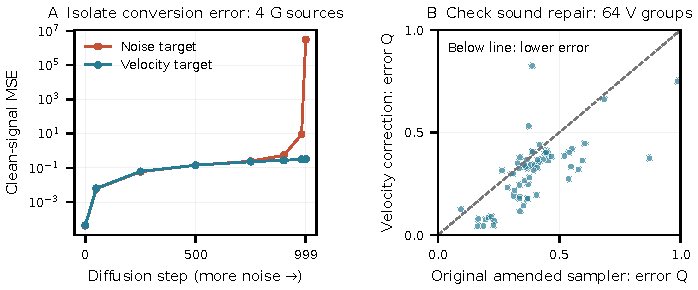
\includegraphics[width=\linewidth]{velocity_correction.pdf}
\caption{Stability and acoustic quality. (A) Reconstruction of known noisy signals on four G recordings at full/reduced precision (solid/dashed). (B) Repair on 64 tuning groups. Below-diagonal points favor correction.}
\label{fig:correction}
\end{figure}

On four G cases, full-precision gap NMSE falls from $5.18\times10^6$ for the terminal sampler to 1.03 for unclipped velocity. Clipping alone gives 22.55, and the original amendment 1.84. The correction removes extreme artificial amplitudes that would otherwise dominate inspection of the repaired sound.

All 192 V groups retain identical gaps and four seeds. Selection uses the first proposal or spectral medoid (most representative frequency pattern). Best-of-four is retrospective. Reserved-development first-proposal Q falls from 0.412 to 0.308, about 25\%. The paired change is $-0.103$ (exploratory 95\% interval $-0.129$ to $-0.077$, 2,000 group-bootstrap draws). Balancing 63 dates gives $-0.104$ ($-0.132$ to $-0.077$).

B still scores better at 0.239. Only 7/64 tuning groups beat B by 0.02 even with best-of-four selection, missing the 20\% trigger. Thus corrected fills better match the withheld sound, but remain too inaccurate to replace B. This follow-up reuses inspected V data, fits no new release rule, and leaves C/test outcomes unopened.

\section{Acoustic evidence behind aggregate scores}

Figure~\ref{fig:acoustic_cases} explains why aggregate improvement needs acoustic inspection. A/B give the original method's best/worst differences from B among 64 reserved cases. C has the most tonal context among seventeen 500 ms gaps. Selection predates correction. C3 uses the selected original proposal, correction its first proposal. Table~\ref{tab:2} also compares first proposals. Class names are dataset annotations.

\begin{figure}[!ht]
\centering
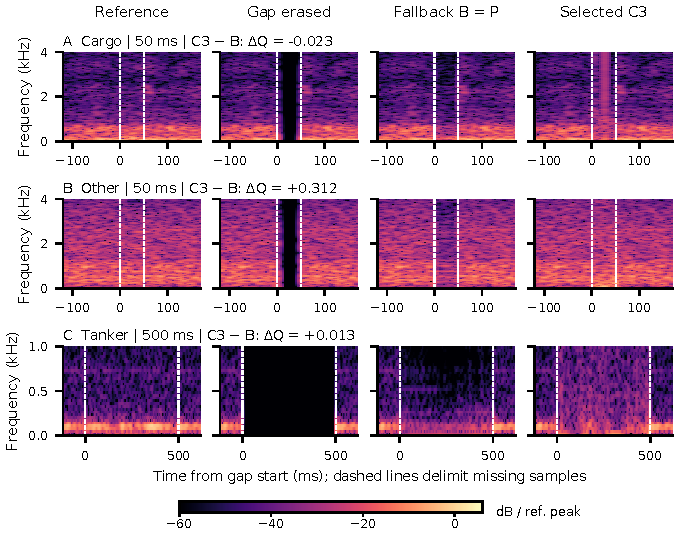
\includegraphics[width=\linewidth]{acoustic_case_studies.pdf}
\caption{Reference, baseline B, original selected C3, and corrected first proposal. Dashed lines mark gaps. Each row shares a brightness scale, and C enlarges low frequencies. The 32 ms windows (4 ms hops) may cross boundaries. References are unavailable during real loss. Corrected proposals are ungated.}
\label{fig:acoustic_cases}
\end{figure}

\noindent\textbf{A. A better score can hide a changed sound pattern.} In the 50 ms cargo gap, C3 lowers Q from B's 0.364 to 0.340 but worsens frequency-pattern error. Correction reduces that error. Inspecting the frequency pattern reveals a change that the combined score hides.

\noindent\textbf{B. A fill can suggest a louder event.} The original 50 ms other-vessel fill is 3.38 dB above reference. Correction is 1.73 dB below. Excess energy and overall error fall, although B remains better. A louder fill cannot establish a stronger recorded event or justify changing recording gain.

\noindent\textbf{C. Restored level can hide the wrong waveform.} A component near 78 Hz continues through the tanker's 500 ms gap. B/C3 underfill overall gap level by 14.48/7.13 dB. Correction is only 1.14 dB below reference, yet Q rises from 0.364 to 0.412. Recovering sound level alone cannot establish what crossed the gap.

In 400 synthetic comparisons, identical available inputs and seeds give identical outputs despite different hidden events. These original-method tests exclude correction and ocean propagation. They illustrate why a fill cannot verify an unobserved event or establish identity.

One seed and shared environments limit interpretation. Three-seed training, waveform RePaint \cite{repaint}, classification, and external validation were not run. Tonal/onset metrics were not fixed in advance, so the examples explain behavior without validating those capabilities.

\section{Measuring verified agent execution}

The second task applies the protocol to agents measuring recorded context and configuring a virtual display. Fixed rules, direct action selection, reasoning, self-review, and a planner--reviewer pair share the task. Inputs are numeric measurements, without audio embeddings, vessel annotations, or generated fills.

A fixed hash order selects 32 V recordings, one per group/date, excluding the anecdotes. Eight tasks each request frequency detail, timing detail, incompatible limits, or fragmented-audio analysis. All hide 500 ms, with additional erasures in fragmented cases. Rules precede responses. Two G transport tests are excluded. Outcomes use development audio.

\textbf{Define the required action.} Longer windows give a finer frequency grid but less precise timing. For $T$ ms, spacing is $1000/T$ Hz, without guaranteeing physical-source separation. Agents choose the shortest feasible 32/64/128/256 ms window with three fully recorded frames per region. Four tools inspect, measure, configure, and read back the result. Twenty tasks permit a change and twelve require refusal.

A \emph{stable} cue requires peaks at least 10 dB above each region's median spectrum, peaks within one selected-window bin, and band levels within 6 dB. A supported comparison outside these limits is \emph{changed}. Weak peaks or no feasible setting give \emph{insufficient}. Hann-window measurements cover 20--600 Hz. Labels describe recorded patterns, without establishing identity or continuity inside gaps.

\textbf{Control the model and allowance.} All neural workflows use Qwen3-8B \cite{qwen3}, BF16, on an RTX PRO 4500. Self-review continues the conversation. A separate reviewer receives task, executed trace, and draft in fresh context, using identical weights without evaluator feedback. Review starts at a draft or four turns, reserving at least half the shared allowance for review. Limits are eight turns, sixteen tool calls, and 6,144 generated tokens, with 512 thinking and 512 action tokens per turn. Capped thinking is closed. Seed 17 has fixed case/turn offsets. Actual costs may differ.

\textbf{Score the completed task.} Success requires correct reported choice and actual state, cue label, supported numbers/citations, post-configuration verification, unknown identity, and intact input/gap flags. Refusal leaves the display unchanged. Citations identify successful tool returns. Fixed rules encode the policy ceiling. All failures are retained. Paired uncertainty uses 10,000 group-bootstrap draws and exact McNemar tests, Holm-adjusted across three predefined contrasts.

\begin{table}[htbp]
\caption{Agent outcomes. Setting checks reported choice and actual state. Complete adds remaining task checks. Tokens gives mean generated length and Seconds median episode time excluding model loading. Primary rows share 32 tasks. Follow-ups are separate.}
\label{tab:3}
\centering\small
\begin{tabular*}{\linewidth}{@{\extracolsep{\fill}}lrrrrr@{}}
\toprule
\textbf{Approach} & \textbf{Setting} & \textbf{Cue} & \textbf{Complete} & \textbf{Tokens} & \textbf{Seconds} \\
\midrule
Fixed rules & 32 & 32 & 32 & 0 & 0.0 \\
Direct agent & 12 & 16 & 10 & 238 & 9.8 \\
Reasoning agent & 18 & 25 & 4 & 3018 & 102.0 \\
Self-review & 16 & 21 & 8 & 3171 & 103.9 \\
Planner--reviewer & 19 & 19 & 9 & 3679 & 134.1 \\
\midrule
\multicolumn{6}{l}{\emph{Feasibility follow-up: 16 new recordings}} \\
Follow-up: reasoning & 8 & 9 & 2 & 3067 & 93.6 \\
Follow-up: guarded & 11 & 9 & 3 & 3122 & 92.8 \\
\midrule
\multicolumn{6}{l}{\emph{Budget check: first 16 primary recordings, reused}} \\
Budget: original & 8 & 13 & 3 & 3044 & 111.6 \\
Budget: longer & 12 & 13 & 5 & 6278 & 187.2 \\
\bottomrule
\end{tabular*}
\end{table}

\textbf{Correct labels can leave acoustic work unfinished.} Reasoning gives 25/32 correct cue labels versus 16/32 for direct mode, yet completes 4/32 tasks versus 10/32. Contrasts of reasoning/direct, self-review/reasoning, and paired agents/self-review are inconclusive after Holm adjustment ($p\geq0.328$). Verification occurs in 5/20 feasible reasoning cases versus 20/20 direct cases. Both review workflows lack drafts at 23/32 handoffs. Ten paired-agent episodes lack valid reports. A correct label can leave the operator with an incorrect or unverified display.

\textbf{Protect frequency and timing detail.} Figure~\ref{fig:configuration} motivates a test on sixteen new groups/dates, four per family. The 8 Hz spacing and 160 ms limits require 128 ms (7.81 Hz), rather than 64 ms (15.63 Hz). Model, prompts, and budgets are matched. One tool rejects infeasible settings without supplying answers or verification.

The gate blocks nine requests, eliminating infeasible applied changes (six to zero). Complete success changes from 2/16 to 3/16 ($+6.25$ percentage points, exploratory 95\% paired interval $[0,18.75]$, exact $p=1$). Both label 9/16 cues correctly and verify 4/10 feasible tasks. Two guarded reports fail solely for citing genuine rejections, excluded by the frozen rule. Display limits are protected, but the operator still needs a completed, verified acoustic assessment.

\textbf{Allow more thinking time.} Frequent truncation (520/585 primary reasoning turns overall) motivates a check on the first sixteen tasks and original controls. The thinking cap rises to 2,048 tokens per turn and total generation to 12,288 tokens. Other settings and scoring stay fixed. No recordings are added.

Turns reaching the limit fall from 87.8\% (79/90 turns) to 27.3\% (21/77). Correct settings rise from 8/16 to 12/16 and complete success from 3/16 to 5/16 ($+12.5$ percentage points, exploratory 95\% interval $[-18.75,43.75]$, exact $p=0.6875$). Generated text roughly doubles, and median time rises from 111.6 to 187.2 s. Two episodes exhaust their allowance. Extra thinking improves some settings at a time cost, without establishing dependable acoustic analysis.

Primary/gate sets each contain one changed cue, with stable/insufficient counts of 16/15 and 3/12. One model/base seed, explicit rules, and reused V audio limit generalization. Paired agents share weights and run sequentially. Gate/budget changes are tested separately. Classification and physical control remain untested.

\section{Conclusion}

Controlled tests separate numerical stability, acoustic fidelity, and verified execution. Velocity prediction lowers reconstruction error by about 25\%, while the baseline advantage and low candidate opportunity identify a remaining modeling problem. Agent traces locate incomplete execution behind correct cue labels. Configuration checks prevent infeasible changes, while extra thinking improves some settings without establishing reliable completion.

These results support marking estimated sound, inspecting level and frequency pattern, and verifying the display used. Frozen inputs and replayable traces make the evaluation reusable. Independent sites, richer cue classes, multiple seeds, identification, and physical trials are needed to establish broader utility.

\clearpage
\paragraph{AI Use Declaration.} OpenAI Codex assisted in the code production, and manuscript draft editing.

\bibliographystyle{splncs04}
\bibliography{references}
\end{document}
